\documentclass[12pt,a4paper,notitlepage]{report}

\renewcommand{\familydefault}{\sfdefault}
% The current University regulation suggests using sans serif font. If this 
% causes you any form of difficulty, feel free to comment out line 3 and the 
% font will switch to roman style.

\usepackage{epcc}
\usepackage{graphicx}
% graphicx, not graphics: \includegraphics[width=...] is keyval syntax and only
% graphicx provides it. The template's plain "graphics" only ever worked here
% because todonotes happened to load TikZ, which loads graphicx behind the scenes.
\usepackage{booktabs}
\usepackage{amsmath}

% Float placement. Without these, the figures of Chapters 4 and 5 queue up and
% are flushed out after the text that discusses them: every section of Chapter 4
% from 4.2 onwards began on the same page, with six figures dumped on the three
% pages after it.
%   placeins  puts a \FloatBarrier before each \section, so a float cannot drift
%             past the section it belongs to.
%   the fractions below let a page carry more float and less text than the
%             defaults allow, which is what a figure-dense chapter needs.
\usepackage{flafter}
% flafter: a float never surfaces on a page BEFORE the point it is declared.
\usepackage[section]{placeins}
% placeins only barriers at \section. The 2D/3D boundary in Chapter 4 is a
% \subsection, so the barrier is lowered one level or a 2D figure drifts past
% the start of the 3D subsection.
\let\OldSubsection\subsection
\renewcommand{\subsection}{\FloatBarrier\OldSubsection}
\renewcommand{\topfraction}{0.9}
\renewcommand{\bottomfraction}{0.8}
\renewcommand{\textfraction}{0.1}
\renewcommand{\floatpagefraction}{0.75}
\setcounter{topnumber}{3}
\setcounter{bottomnumber}{2}
\setcounter{totalnumber}{5}

% This example file shows how a thesis can be laid out using Latex. It
% does not use any special local features so should be portable to other
% places.
% 
% This document contains many cross-references and forward references,
% eg in constructing a table of contents, so Latex may need to be run
% twice to get all the references correct. If you need to run Latex twice
% you may get the warning:
% 
% LaTeX Warning: Label(s) may have changed. Rerun to get cross-references right.

%\usepackage{todonotes}
% Commented out: todonotes pulls in the whole of TikZ/PGF, which is by far the
% slowest thing in this preamble, and nothing in this document uses \todo.
% Uncomment it if you start leaving notes for yourself.
% The to-do notes package
% [http://tug.ctan.org/macros/latex/contrib/todonotes/todonotes.pdf] 
% is not needed for typesetting your final report, however, you may find it
% useful when drafting it. You can leave notes for yourself or your 
% proof-reader using 
%   \todo{Your note here} -- this will put the note's text into the margin
%   \todo[inline]{An inline note} -- this will show as a line in your document


\usepackage{iftex}
\ifPDFTeX
  \usepackage[utf8]{inputenc}
  \usepackage[T1]{fontenc}
  \usepackage{lmodern}
\fi

\usepackage[backend=biber,style=numeric,sorting=none]{biblatex}
\addbibresource{references.bib}

\usepackage[hidelinks]{hyperref}
% to allow clickable references
\usepackage{cleveref}

\begin{document}
\indentedparagraphing


% Author- and Report-specific information
% DO CHANGE THIS BIT!
%
\title{Hybrid MPI+OpenMP Performance of PETSc on ARCHER2}
\author{Leyan li}
\date{Date} 
	% you should use an unambiguous date format, such as Day(number) Month(word) Year(number), 
	% or you can use \date{\today} for the current date


\makeEPCCtitle 
% This takes care of creating all the logos on the title page as described in
% epcc.sty --- feel free to explore it!

\thispagestyle{empty} 
% We don't want any page numbers, headers or footers on the title page,
% hence "empty" style.

% The below is a dirty way of adding all the relevant degree- and university- 
% information onto the title page. Sorry.
%
\vspace{5cm} % This controls the amount of vertical space between the title and 
			 % your name, and the degree information. The University, degree and 
			 % year should show at the bottom of the page so please adjust 
			 % the vspace accordingly, to avoid it overflowing onto the next page.

\begin{center}

% Adjust the information below to fit your situation. If anything takes more 
% space than expected in the template, adjust spacing above/below to keep all
% this on the first page.
\large{MSc in High Performance Computing (with Data Science)} \\ 
	% update based on your degree
\large{The University of Edinburgh} \\ %
\large{2026} \\ % update to the year you are submitting your dissertation 

\end{center}

% This is it, the title page is done. Go you!

% We are starting to number pages from here, right after the title page.
% These are non-technical content pages, and these are 
% number them with roman numerals. Content pages (starting from
% Chapter 1) will get numbered with arabic numerals, restarting from '1'.
\pagenumbering{roman}
\setcounter{page}{0}
\newpage

% We used the "abstract" style common in research publications and
% therefore use the predefined LaTeX macro. However, we want this page
% to be numbered with 'i' (first page after the title), so we need to
% overwrite the page style to show page numbers, adding 
% \thispagestyle{plain} **inside** the abstract.
\begin{abstract} 
\thispagestyle{plain}
\noindent This is the bit where you summarise what is in your thesis. A non-expert reader 
should be able to understand the area of your work, what the main challenges 
were and what contributions or insights you've achieved, and gauge whether 
this work is relevant to their interests,. Think of the abstract as 
a super-concentrated summary of your MSc project; advertise your work 
but try to avoid cliffhangers.

A good abstract fits to 1 to 2 paragraphs and takes around 200 words to get your 
point across. To give you an idea, this abstract is 97 words long.
\end{abstract}


% The following commands generate pages of non-technical content; as the names 
% suggest, we will generate tables of content, of tables and of figures. It is 
% recommended that you have a look at these tables and decide whether they are 
% displayed correctly with a meaningful amount of information (for example,
% list of figures should not contain the full figure captions), and whether 
% they are relevant and needed.
%
\tableofcontents
\listoftables
\listoffigures

% You may decide to include additional sections, for example the 
% Acknowledgements or Dedications. Make sure these start on a new page, 
% following the structure below:
\newpage

% This vspace is just to avoid having a short amount of text 
% (the Acknowledgements) hanging awkwardly at the very top of the page.
\vspace*{2in}

\section*{Acknowledgements}

Here you can give credit to anyone who has enabled the progress of your MSc 
project, especially if this was \emph{above and beyond} their role. Below is 
our acknowledgement of the people who contributed to creation of this template. 
\\ \\
%
This template is a slightly modified version of the one developed by
Prof. Charles Duncan for MSc students in the Dept. of Meteorology. His
acknowledgement follows:

\emph{This template has been produced with help from many former students who
have shown different ways of doing things. Please make suggestions for
further improvements.} 
% This is the end of the "initial matters", the technical content follows
% from here. The page numbering is restarted and arabic style invoked 
% by the command below.
%
\cleardoublepage
\pagenumbering{arabic}
% The template describes this line but never had it: without it the whole
% document stays in roman numerals and Chapter 1 opens on page xviii.



%%%%%%%%%%%%%%%%%%%%%%%%%%%%%%%%%%%%%%%%%%%%%%%%%%%%%%%%%%%%%%%%%%%%%%%%%%%%%%%

\chapter{Introduction}
\label{ch:intro}
% Write last, once contributions are final.

\section{Motivation}
\label{sec:motivation}
% PETSc depends on MPI; flat-MPI limits on many-core NUMA nodes; PETSc OpenMP backend.

\section{Aims and Research Questions}
\label{sec:aims}
This study measures PETSc rank--thread configurations for a Poisson problem on ARCHER2:
flat MPI against hybrid MPI+OpenMP, in 2D and 3D, at four problem sizes, from 1 to 64
nodes. It asks whether hybrid execution reduces runtime, which configuration gives the
lowest runtime, and where the time goes.


\section{Contributions}
\label{sec:contributions}
%	1. Systematic rank-thread sweep of 2D/3D KSP benchmarks on ARCHER2.
%	2. A reproducible experimental framework.
%	3. A profiling-driven bottleneck-localisation method (RepeatedSolves + MAP + log\_view).

\section{Dissertation Structure}
\label{sec:structure}


\chapter{Background and Related Work}


\section{Parallel Programming Models}
A hybrid program assigns one or more MPI ranks to each node and creates an OpenMP team
inside every rank.
\begin{table}[htbp]
  \centering
  \caption{The three execution models as they apply within one ARCHER2 node. The hybrid
  row is the subject of this dissertation; it inherits both cost columns.}
  \label{tab:models}
  \begin{tabular}{l p{0.20\textwidth} p{0.21\textwidth} p{0.34\textwidth}}
    \toprule
    Model & Memory & Data exchange & Principal cost \\
    \midrule
    MPI    & Private per rank
           & Explicit messages
           & Message matching, per-rank solver state, one subdomain boundary per rank \\
    \addlinespace
    OpenMP & Shared within a team
           & Shared addresses
           & Team creation, synchronisation, cache and bandwidth contention \\
    \addlinespace
    Hybrid & Shared inside a rank, private between ranks
           & Messages between ranks only
           & Both, traded against each other by the rank--thread balance \\
    \bottomrule
  \end{tabular}
\end{table}


\section{Limitations of Flat MPI}
Flat MPI assigns one rank to each core.

\section{Hybrid MPI+OpenMP}
\label{sec:hybrid}
PETSc --with-openmp-kernels

\section{ARCHER2 Node Architecture and NUMA}
\label{sec:archer2}
% Reuse archer2.png. 2x AMD EPYC 7742, 128 cores, 8 NUMA regions.
An ARCHER2 compute node has two AMD (Rome) processors,  giving 128 physical cores.
The service configures four NUMA regions per socket, eight per node, each with 16 cores and local memory
channels in each region. A core has private L1 and L2 caches. Four cores forms a
Core Complex (CCX) and share a 16MB L3 cache, two CCXs form a Core Complex Die (CCD). 
Different CCXs do not share L3 cache \cite{archer2_hardware}.

\begin{figure}[htbp]
    \centering
    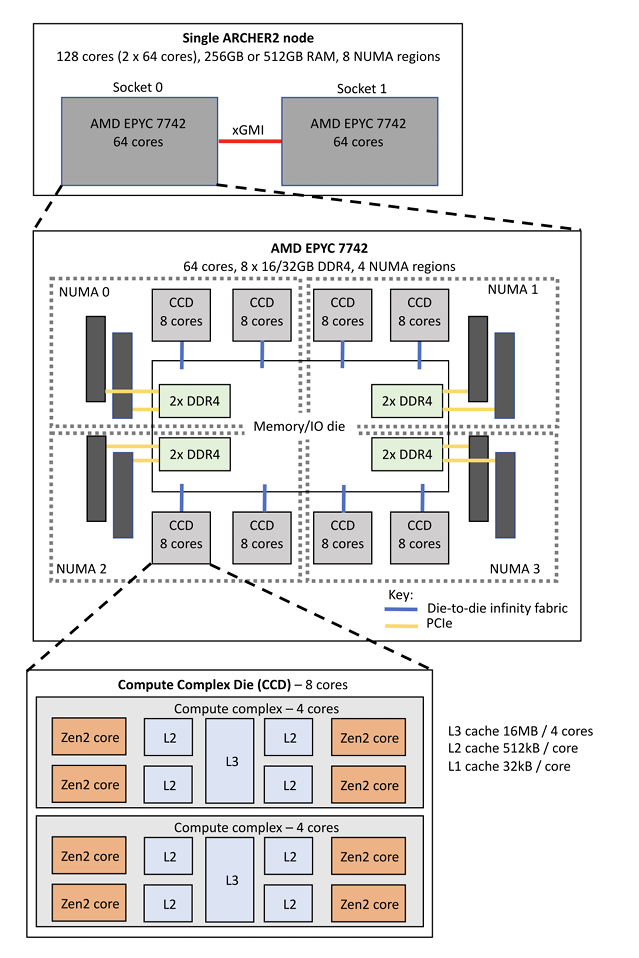
\includegraphics[width=0.4\textwidth]{figures/archer2.png}
    \caption{Architecture of an ARCHER2 node, consisting of two 64-core AMD EPYC 7742 processors.}
    \label{fig:archer2_architecture}
\end{figure}

NUMA affects each both latency and bandwidth. Linux normally allocates a page in the NUMA
region of the thread that first touches it. If a thread creates a large array and a team
accesses it later later from several regions, remote traffic can concentrate on the memory controllers
of the first region. The ARCHER2 guide also notes that two threads can approach the memort-bandwidth limit 
of a NUMA region for bandwidth-intensive code \cite{archer2_tuning}.
More threads do not guarantee more bandwidth.

Cache topology introduces a finer boundary than NUMA. Four adjacent cores share an
L3 cache, whereas a 16-core NUMA region countains four such L3 caches. With close binding,
$32\times4 $ can place one four-thread rank within on CCX; $64\times2$ can use two 
two-thread rank to share one CCX. $16\times8$ can make a rank span two CCXs, 
and $128\times1$ can make a rank span the whole node. This mapping is a plausible mechainism
for layout differences, The experiment fix thread affinity and compare measuremetns before
using topology to interpret the results, The relevant binding options are:

\begin{verbatim}
--cpu-bind=cores
--distribution=block
--hint=nomultithread
\end{verbatim}

\section{PETSc and Krylov Solvers}
\label{sec:petsc-krylov}

PETSc provides distributed vectors and matrices, Krylov solvers (KSP), preconditioners (PC), and a built-in logging system.
It talks between processes with MPI, and it lets the user pick solver components at run time.

\section{Performance Analysis Tools}
\label{sec:tools}

\texttt{log\_view} and Linaro MAP are the two PETSc tools used in this study.
\texttt{log\_view} is a built-in logging system that can report the time spent in each PETSc function,
while Linaro MAP is a sampling profiler for MPI, OpenMP, and single-threaded programs
that provides detailed information about the performance of PETSc applications,
including memory usage, communication patterns, and computational efficiency.




\section{Summary and Research Gap}
\label{sec:gap}

\section{Dissertation Report}


\chapter{Experimental Platform and Methodology}
\label{ch:methodology}


\section{Hardware and Software Environment}
\label{sec:env}
All experiments ran on ARCHER2. Each node has two AMD EPYC 7742 processors, 128 physical
cores, and eight NUMA regions of 16 cores each. The software stack was PrgEnv-gnu 8.4.0,
gcc 11.2.0, and cray-mpich 8.1.27. PETSc 3.24.4 was built from source as
\texttt{arch-omp-opt}. The repeated-solve campaigs used
\texttt{arch-omp-libsci-rome-opt}, configured with the threaded \texttt{libsci\_gnu\_mp.so.5.0} .
Both with PETSC`s OPENMP kernels and use \texttt{-O3}.
One thread per rank is used as the MPI-only baseline. 





\section{Benchmark Problems and Drivers}
\label{sec:benchmarks}
The 2D benchmark is PETSc \texttt{ex2}, a five-point stencil discretisation of the Laplace
operator on an $m \times n$ grid. The 3D benchmark is a driver written for this project, a
seven-point stencil on an $m \times n \times p$ grid; it was added because
surface-to-volume ratio differs from 2D. Its production driver,
\texttt{ex2\_repeat}, separates one warm-up solve from 19 timed solves with a reused
preconditioner (\Cref{ch:profiling}). The matched \texttt{3d\_repeat} driver applies the
same measurement design to a seven-point stencil on an $m \times n \times p$ grid.

\section{Solver Configuration}
The default \texttt{ex2} solver is GMRES with block Jacobi.Block Jacobi builds one block per MPI rank, so the preconditioner is a function of the rank
decomposition: changing the rank--thread layout changes the operator that is applied.
The dependence is not monotonic in the rank count, so it cannot be read as a
trade-off between preconditioner strength and parallelism either. Two layouts with
different rank counts apply different preconditioners to the same linear system, and a
wall-clock difference between them reflects that difference as much as any property of the
layout. Cross-layout runtime under this solver is therefore indicative only, and the
question ``which rank--thread layout is fastest?'' has no well-posed answer.
\Cref{tab:iterations-rank} shows this directly. Reading across any row, the iteration count
does not change at all when threads are added; reading down any column, it changes by a
factor of more than three.

\begin{table}[htbp]
  \centering
  \caption{Final iteration count of the single-node default-solver sweep on a
  $1000\times1000$ grid, for every $\text{ranks}\times\text{threads}\leq128$ combination.
  Every row is constant: the count is fixed by the rank count alone. The 128-rank
  configuration reached the 10,000-iteration limit without converging.}
  \label{tab:iterations-rank}
  \begin{tabular}{lrrrrrrrr}
    \toprule
    & \multicolumn{8}{c}{OpenMP threads per rank} \\
    \cmidrule(lr){2-9}
    MPI ranks & 1 & 2 & 4 & 8 & 16 & 32 & 64 & 128 \\
    \midrule
    1   &  6700 & 6700 & 6700 & 6700 & 6700 & 6700 & 6700 & 6700 \\
    2   &  3715 & 3715 & 3715 & 3715 & 3715 & 3715 & 3715 &      \\
    4   &  2825 & 2825 & 2825 & 2825 & 2825 & 2825 &      &      \\
    8   &  4085 & 4085 & 4085 & 4085 & 4085 &      &      &      \\
    16  &  8179 & 8179 & 8179 & 8179 &      &      &      &      \\
    32  &  6460 & 6460 & 6460 &      &      &      &      &      \\
    64  &  7181 & 7181 &      &      &      &      &      &      \\
    128 & 10000 &      &      &      &      &      &      &      \\
    \bottomrule
  \end{tabular}
\end{table}





CG is used because it is a common Krylov method for symmetric positive definite problems, 
and GAMG removes that coupling. 
\begin{verbatim}
-ksp_type cg -pc_type gamg -ksp_rtol 1e-5 -ksp_atol 1e-10
\end{verbatim}
Its iteration count is set by the multigrid hierarchy and not
by the rank decomposition.


GAMG cost has two pahase: set up(\texttt{PCSetUp}) and solve (\texttt{KSPSolve}). 
The setup phase is more expensive than the solve phase. In a single run, setup is about 45\% of the run time,
and the cost is amortised over multiple solves. 
Therefore, the profiling uses repeated solves (19 times) to measure the performance of the solver. 
The total time including setup and solve is measured, \Cref{ch:profiling} isolates the solve phase.



\section{Configuration Space and Selection Rules}
\label{sec:configspace}
Three rules are followed in this experiment:

1.Threads per rank are restricted to $\{1,2,4,8\}$. 

2.Nodes are fully populated: $\text{ppn} \times \text{threads} = 128$, giving four layouts
$128\times1$, $64\times2$, $32\times4$, and $16\times8$. Same node count means same core
count, so a comparison isolates rank--thread balance from core count.

3.A configuration at size $N$ on $C$ physical cores is included when
$25{,}000 \leq N/C \leq 100{,}000$. The completed 2D campaign uses six grids:
$2240^2$, $3160^2$, $4500^2$, $6400^2$, $9073^2$, and $12828^2$, or 5.02M to
164.56M unknowns.



\section{Job Configuration and Thread Placement}
\label{sec:placement}
Each rank and its threads are pinned to a contiguous set of cores with:
\begin{verbatim}
OMP_PLACES=cores   OMP_PROC_BIND=close
srun --hint=nomultithread --distribution=block:block --exact
\end{verbatim}

The primary timing is the maximum-rank \texttt{KSPSolve} time in the
\texttt{RepeatedSolves} stage. If this event has count $c=19$, time $t$, and the grid has
$N$ unknowns, steady-state throughput is
\[
  Q = \frac{Nc}{t}.
\]
The analysis also reports $t/(cI)$, where $I$ is the final KSP iteration count. Formal
repeats are aggregated by their median; whiskers show the observed minimum and maximum
from three runs. Scaling is computed per layout against that layout's smallest admitted
node count. For a layout $\ell$ at $n$ nodes,
\[
  S_\ell(n) = \frac{T_\ell(n_0)}{T_\ell(n)}, \qquad
  E_\ell(n) = \frac{S_\ell(n)}{n/n_0},
\]
where $n_0$ is the smallest node count run for that problem size.

\chapter{2D and 3D Problems}
\label{ch:multinode}

\section{Experimental Setup}
\label{sec:mn-setup}
Two campaigns cover each dimension. Both use the platform, build, solver and thread
placement of \Cref{ch:methodology}, and both fill every node with all 128 cores. They
differ in one thing. The weak-scaling campaign grows the problem with the node count. The
fixed-size campaign holds it still. \Cref{tab:fullnode-matrix} lists both.

\begin{table}[htbp]
  \centering
  \caption{Grids and node counts of the six scales. The fixed-size column is not limited by the
  filter of \Cref{sec:configspace}.}
  \label{tab:fullnode-matrix}
  \small
  \begin{tabular}{lrrrrll}
    \toprule
    Scale & 2D grid & 2D unknowns & 3D grid & 3D unknowns & Weak-scaling & Fixed-size \\
          &         &             &         &             & nodes        & nodes \\
    \midrule
    5m   & $2240^2$  &   5,017,600 & $171^3$ &   5,000,211 & 1      & --- \\
    10m  & $3160^2$  &   9,985,600 & $215^3$ &   9,938,375 & 1, 2   & --- \\
    20m  & $4500^2$  &  20,250,000 & $273^3$ &  20,346,417 & 2, 4   & 1, 2, 4, 8, 16, 32 \\
    41m  & $6400^2$  &  40,960,000 & $345^3$ &  41,063,625 & 4, 8   & --- \\
    82m  & $9073^2$  &  82,319,329 & $435^3$ &  82,312,875 & 8, 16  & --- \\
    165m & $12828^2$ & 164,557,584 & $548^3$ & 164,566,592 & 16, 32 & --- \\
    \bottomrule
  \end{tabular}
\end{table}

That gives 11 size--node pairs in the weak-scaling campaign and six in the fixed-size one.
Every pair runs all four layouts three times. All 280 weak-scaling logs and all 144
fixed-size logs passed the content checks. None carries a divergence, a PETSc or MPI
error, or a licence wait.

Run-to-run spread limits what can be resolved. Over three repeats the largest spread is
4.71\% in 2D and 3.83\% in 3D for the weak-scaling matrix. For the fixed-size curves it is
10.77\% and 11.09\%, because a solve at the largest node counts takes only tens of
milliseconds. A gap smaller than these is reported as a tie. Whiskers in the figures show the
observed range of the three runs.

\subsection{Weak-Scaling Chains}
\label{sec:bands}
The filter $25{,}000 \leq N/C \leq 100{,}000$ admits each scale at only one or two node
counts, so a panel drawn per problem size holds two points. The same 11 pairs split into
two chains of near-constant unknowns per core (\Cref{tab:bands}). Ideal weak scaling would
hold the time per iteration flat along a chain. The measured rise is the cost of
concurrency.

\begin{table}[htbp]
  \centering
  \caption{The 11 admitted size--node pairs, ordered into two weak-scaling chains.}
  \label{tab:bands}
  \begin{tabular}{lllllll}
    \toprule
    Band & \multicolumn{6}{c}{Size at node count} \\
    \cmidrule(lr){2-7}
         & 1 & 2 & 4 & 8 & 16 & 32 \\
    \midrule
    $\sim$40k unknowns/core & 5m & 10m & 20m & 41m & 82m & 165m \\
    $\sim$80k unknowns/core & 10m & 20m & 41m & 82m & 165m & --- \\
    \bottomrule
  \end{tabular}
\end{table}

\subsection{Strong-Scaling Design}
\label{sec:strong20m}
The chains span one node doubling per problem size. That cannot show where a layout stops
scaling. A second campaign therefore fixes the 20m problem and runs the full sequence
$\{1,2,4,8,16,32\}$ nodes, with nothing else changed. At 32 nodes this leaves about 4.9
thousand unknowns per core, below the admission window. That point is the saturation tail
and not a sensible operating point.

\section{Weak Scaling at Constant Work per Core}
\label{sec:weak}
Both dimensions run the same 11 pairs, the same four layouts and the same three repeats.

\subsection{2D}
\label{sec:weak-2d}
Throughput rises almost linearly with the node count (\Cref{fig:2d-throughput}). All four
layouts sit within a few per cent of each other on that axis, so it cannot separate them.
\Cref{fig:2d-ratio} divides each layout's time per iteration by that of flat MPI at the
same size--node pair. This removes the scale and the GAMG iteration count and leaves the
layout effect.

\begin{figure}[htbp]
  \centering
  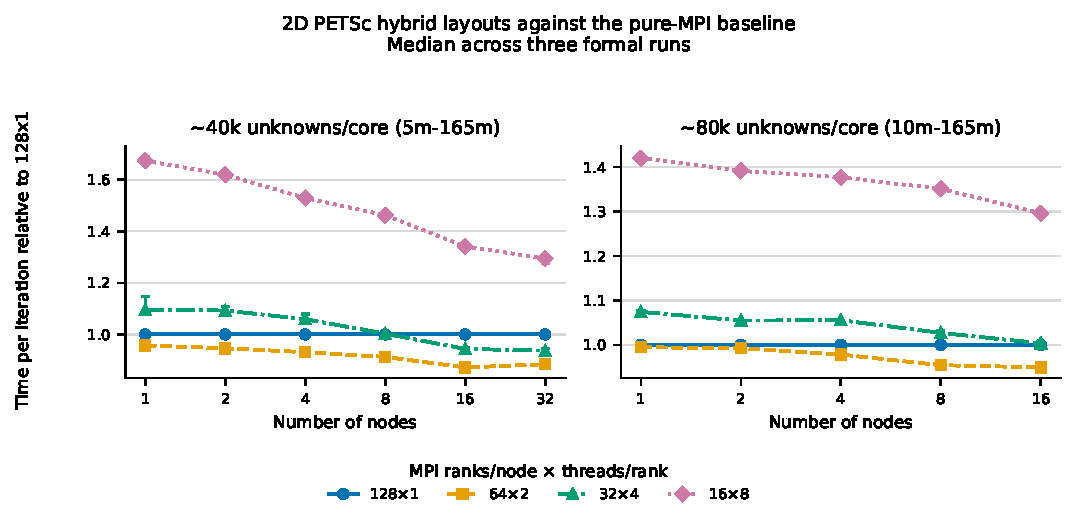
\includegraphics[width=\textwidth]{figures/ksp2d_layout_vs_mpi}
  \caption{2D time per KSP iteration relative to the $128\times1$ baseline. Values below 1 mean
  the hybrid layout is faster.}
  \label{fig:2d-ratio}
\end{figure}

The curves fall. Along the $\sim$40k chain $64\times2$ goes from 0.957 at one node to
0.872 at 16, and $32\times4$ from 1.096 to 0.937. Along the $\sim$80k chain all three
hybrid ratios drop at every step. Four of the six series are strictly monotone.

Two things follow. $64\times2$ beats flat MPI per iteration at all 11 pairs, and its lead
grows with the node count. $32\times4$ starts 9.6\% behind flat MPI, reaches parity at
eight nodes, and is 6.3\% ahead at 32 nodes. A ranking taken at one node does not hold at
32.

$16\times8$ is the slowest layout at every pair. Its deficit does narrow, from 46.2\% at
5m on one node to 22.7\% at 165m on 32 nodes.

\Cref{fig:2d-spi} gives the absolute time per iteration. A flat line would be ideal weak
scaling.

\begin{figure}[htbp]
  \centering
  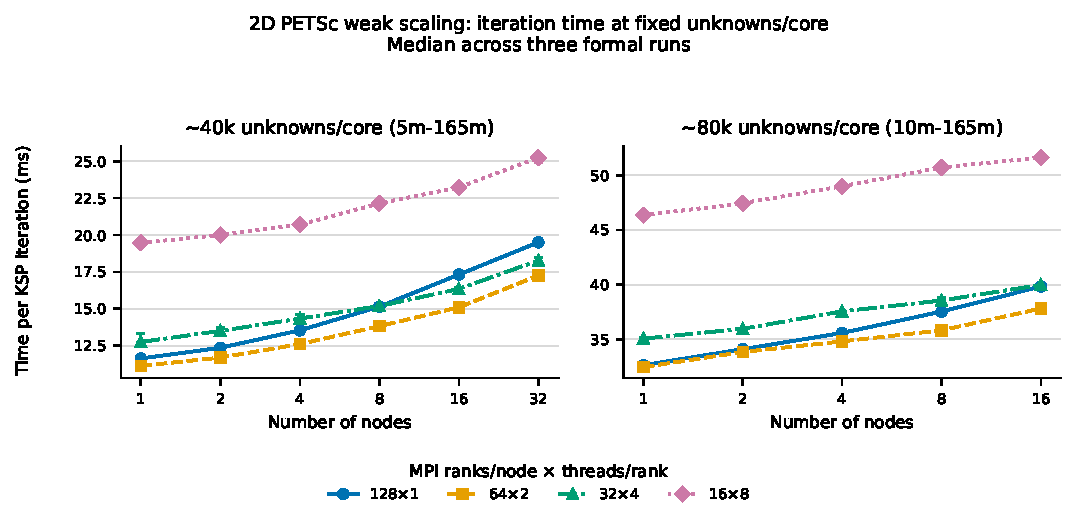
\includegraphics[width=\textwidth]{figures/ksp2d_seconds_per_iteration}
  \caption{Median 2D time per KSP iteration along the two unknowns/core chains.}
  \label{fig:2d-spi}
\end{figure}

\subsection{3D}
\label{sec:weak-3d}
The 3D campaign uses the same points, layouts and repeats. Its throughput has the same
near-linear shape (\Cref{fig:3d-throughput}), so the comparison again uses the ratio
(\Cref{fig:3d-ratio}).

\begin{figure}[htbp]
  \centering
  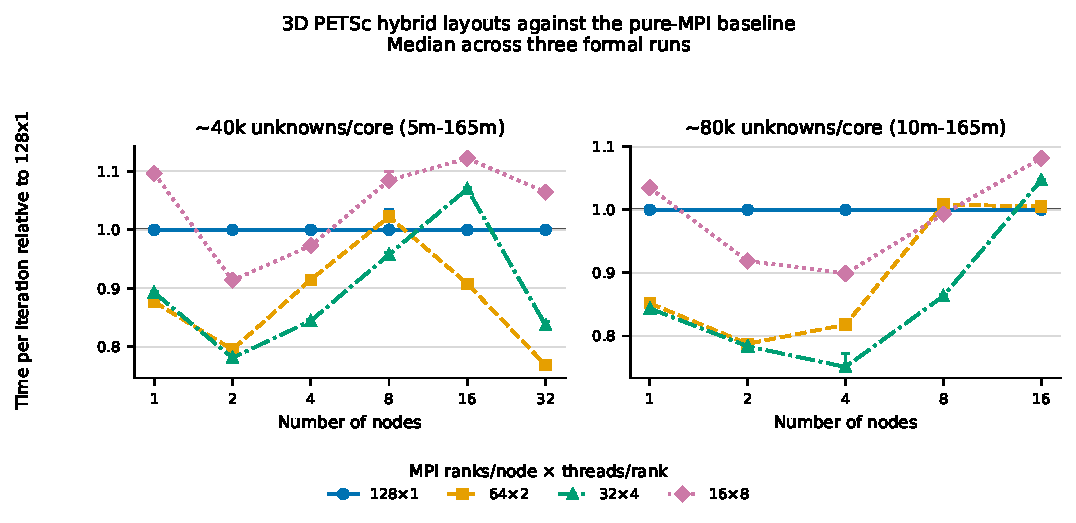
\includegraphics[width=\textwidth]{figures/ksp3d_layout_vs_mpi}
  \caption{3D time per KSP iteration relative to the $128\times1$ baseline. Unlike 2D, no series
  is monotone.}
  \label{fig:3d-ratio}
\end{figure}

3D differs from 2D in size and in shape. The best point is $32\times4$ at 41m on four
nodes, at a ratio of 0.751. That is 24.9\% less time per iteration than flat MPI, against
a 2D best of 12.8\%. Of the 33 hybrid measurements 22 fall below 1, against 13 of 33 in
2D.

The shape differs too. None of the six series is monotone. On the $\sim$80k chain the
hybrid layouts lead at two and four nodes, lose the lead by eight nodes, and are at or
above parity at 16. On the $\sim$40k chain $64\times2$ rises to 1.022 at 41m on eight
nodes and then falls back to 0.768 at 165m on 32.

$16\times8$ wins no point. Unlike the 2D case it is not always last, and it beats flat MPI
at five of the 11 pairs.

\Cref{fig:3d-spi} gives the absolute time per iteration, on the same convention as the 2D
case.

\begin{figure}[htbp]
  \centering
  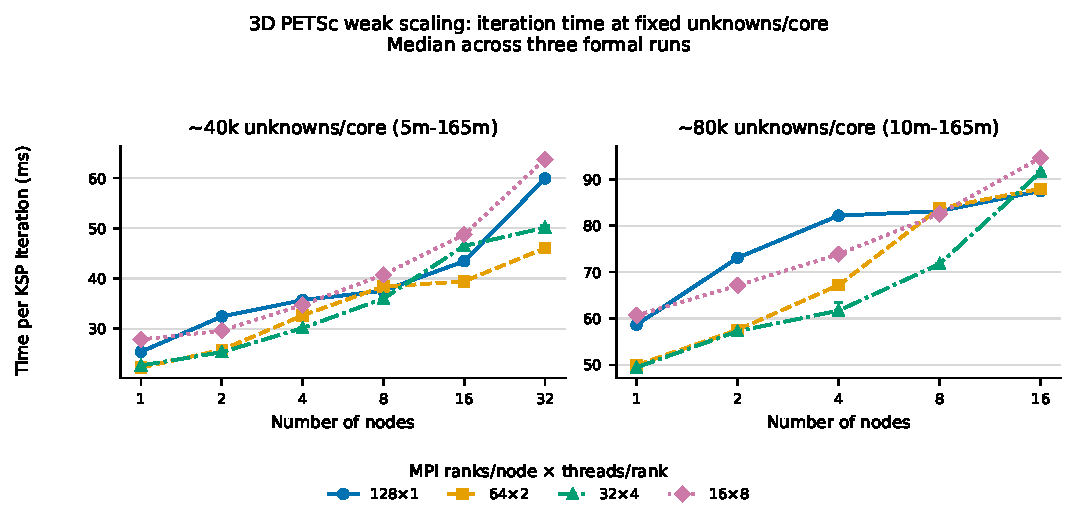
\includegraphics[width=\textwidth]{figures/ksp3d_seconds_per_iteration}
  \caption{Median 3D time per KSP iteration along the two unknowns/core chains.}
  \label{fig:3d-spi}
\end{figure}

\subsection{Layout Ranking and Efficiency}
\label{sec:weak-ranking}
\Cref{tab:weak-best} gives the fastest layout at every pair and its margin over flat MPI.

\begin{table}[htbp]
  \centering
  \caption{Fastest full-node layout at every admitted size--node pair, by median throughput. A
  margin of 0.0\% means flat MPI was fastest.}
  \label{tab:weak-best}
  \small
  \begin{tabular}{lrrlrrr}
    \toprule
    Scale & Nodes & Cores & Best layout & M eq/s & vs.\ MPI & ms/iteration \\
    \midrule
    \multicolumn{7}{l}{\emph{2D, five-point stencil}} \\
    5m   &  1 &  128 & $128\times1$ &  47.9 &  0.0\% & 11.63 \\
    10m  &  1 &  128 & $128\times1$ &  34.0 &  0.0\% & 32.63 \\
    10m  &  2 &  256 & $64\times2$  &  94.9 &  5.7\% & 11.69 \\
    20m  &  2 &  256 & $64\times2$  &  59.8 &  0.8\% & 33.84 \\
    20m  &  4 &  512 & $64\times2$  & 160.7 &  7.4\% & 12.60 \\
    41m  &  4 &  512 & $64\times2$  & 107.0 &  2.2\% & 34.81 \\
    41m  &  8 & 1024 & $128\times1$ & 270.5 &  0.0\% & 15.14 \\
    82m  &  8 & 1024 & $64\times2$  & 208.9 &  4.8\% & 35.82 \\
    82m  & 16 & 2048 & $64\times2$  & 495.6 & 14.7\% & 15.10 \\
    165m & 16 & 2048 & $64\times2$  & 362.6 &  5.3\% & 37.82 \\
    165m & 32 & 4096 & $64\times2$  & 794.8 & 13.1\% & 17.25 \\
    \addlinespace
    \multicolumn{7}{l}{\emph{3D, seven-point stencil}} \\
    5m   &  1 &  128 & $64\times2$  &  37.4 & 14.1\% & 22.26 \\
    10m  &  1 &  128 & $32\times4$  &  28.7 &  1.6\% & 49.45 \\
    10m  &  2 &  256 & $64\times2$  &  64.3 & 25.8\% & 25.78 \\
    20m  &  2 &  256 & $32\times4$  &  50.8 & 27.6\% & 57.26 \\
    20m  &  4 &  512 & $32\times4$  &  96.5 &  1.5\% & 30.13 \\
    41m  &  4 &  512 & $32\times4$  &  95.1 & 33.2\% & 61.68 \\
    41m  &  8 & 1024 & $32\times4$  & 163.0 &  4.4\% & 35.99 \\
    82m  &  8 & 1024 & $32\times4$  & 163.9 & 15.8\% & 71.75 \\
    82m  & 16 & 2048 & $64\times2$  & 298.2 & 10.2\% & 39.44 \\
    165m & 16 & 2048 & $128\times1$ & 268.8 &  0.0\% & 87.47 \\
    165m & 32 & 4096 & $64\times2$  & 510.4 & 30.1\% & 46.06 \\
    \bottomrule
  \end{tabular}
\end{table}

$64\times2$ wins 8 of the 11 2D pairs. In 3D $32\times4$ wins 6, $64\times2$ wins 4 and
flat MPI wins 1. The 2D winner changes twice down the column and the 3D winner changes
five times. 2D has one layout ahead throughout. 3D does not. One of the three 2D flat-MPI wins,
41m on eight nodes, is a tie: the medians differ by 0.4\% and the ranges overlap.

\Cref{tab:weak-eff} measures each layout against its own one-node time.

\begin{table}[htbp]
  \centering
  \caption{Weak-scaling efficiency (\%) at the largest node count of each chain, against each
  layout's own one-node time.}
  \label{tab:weak-eff}
  \begin{tabular}{llrrrr}
    \toprule
    & & \multicolumn{4}{c}{Layout} \\
    \cmidrule(lr){3-6}
    Case & Chain and node count & $128\times1$ & $64\times2$ & $32\times4$ & $16\times8$ \\
    \midrule
    2D & $\sim$40k, 32 nodes & 59.6 & 64.5 & 69.8 & 77.1 \\
    2D & $\sim$80k, 16 nodes & 81.9 & 85.8 & 87.7 & 89.8 \\
    3D & $\sim$40k, 32 nodes & 42.4 & 48.3 & 45.2 & 43.7 \\
    3D & $\sim$80k, 16 nodes & 67.0 & 56.8 & 54.0 & 64.1 \\
    \bottomrule
  \end{tabular}
\end{table}

In 2D the ordering is strict in both chains. Efficiency rises with threads per rank, and
$16\times8$ degrades least of the four. In 3D there is no such ordering. On the $\sim$40k
chain $64\times2$ degrades least, and on the $\sim$80k chain flat MPI does.

This is not a statement about speed. $16\times8$ has the best 2D efficiency and the worst
2D time at every point. It degrades least because its cost is already dominated by a term
that does not grow with the node count. Efficiency measured against a layout's own
baseline rewards a bad baseline.

\section{Strong Scaling at Fixed Problem Size}
\label{sec:strong}

\subsection{2D}
\label{sec:strong-2d}
The 2D curves scale well and stay together (\Cref{fig:2d-strong20m}). Every layout is
still improving at 32 nodes. The spread between fastest and slowest goes from
$1.47\times$ at one node to $1.81\times$ at 16 and back to $1.48\times$ at 32.
$64\times2$ and flat MPI finish within 2\% of each other. $16\times8$ starts 47\% behind
and ends 45\% behind.

\begin{figure}[htbp]
  \centering
  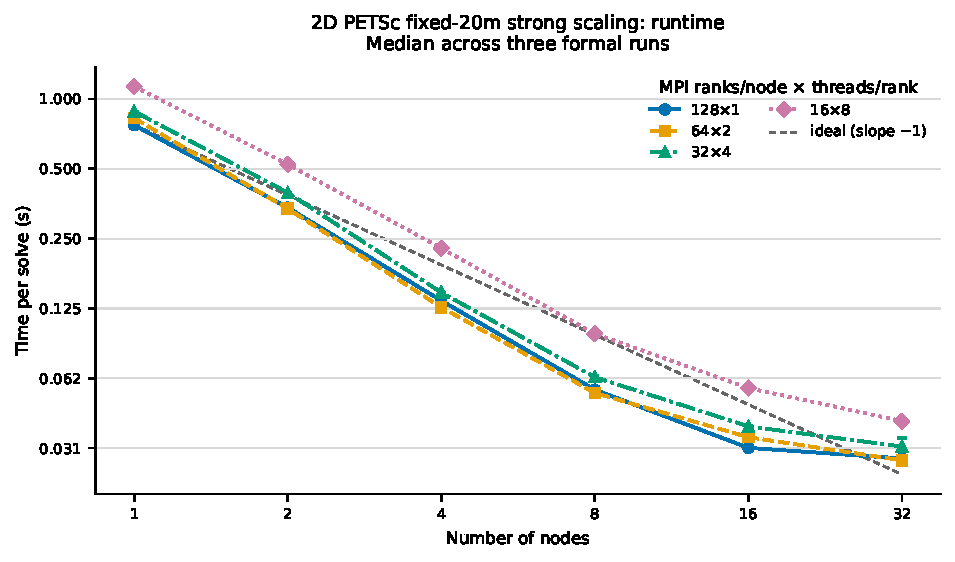
\includegraphics[width=0.85\textwidth]{figures/ksp2d_strong20m_runtime}
  \caption{2D time per solve at a fixed 20.25M unknowns. Both axes are logarithmic, so ideal
  strong scaling has slope $-1$.}
  \label{fig:2d-strong20m}
\end{figure}

Cumulative efficiency passes 100\% between two and 16 nodes and peaks at 191\% for
$64\times2$ at eight nodes. These superlinear values repeat across the three runs. This
experiment does not explain them. The fixed problem shrinking into cache is one candidate
it cannot test.

\subsection{3D}
\label{sec:strong-3d}
The 3D result is different in kind, and it is the largest layout effect in this study
(\Cref{fig:3d-strong20m}). Every 3D layout eventually turns and gets slower. They turn at
different node counts, and the order is the thread count.

\begin{figure}[htbp]
  \centering
  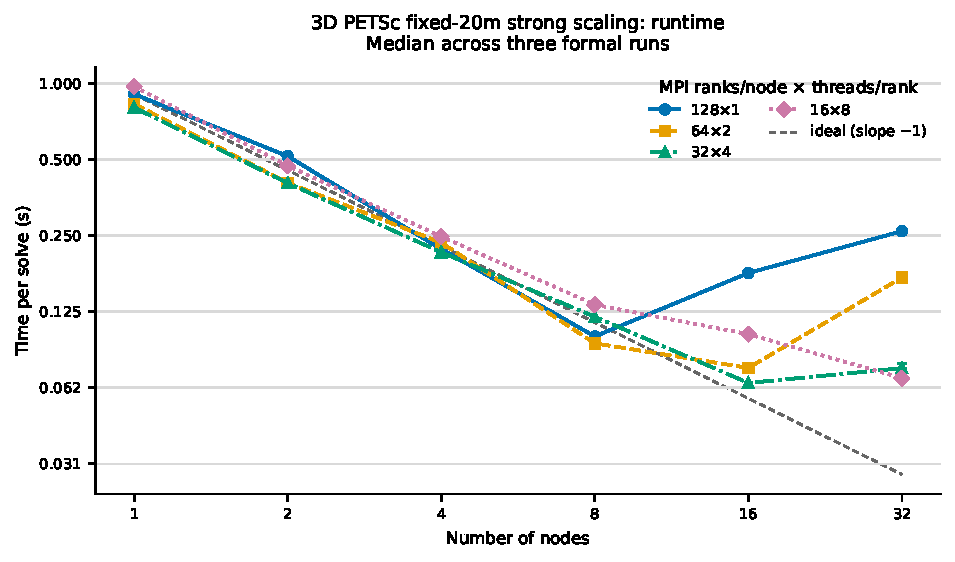
\includegraphics[width=0.85\textwidth]{figures/ksp3d_strong20m_runtime}
  \caption{3D time per solve at a fixed 20.35M unknowns. Flat MPI and $64\times2$ turn and get
  slower; the most-threaded layouts do not.}
  \label{fig:3d-strong20m}
\end{figure}

Flat MPI turns first. It bottoms at eight nodes with 0.0997\,s per solve, then rises to
0.1776\,s at 16 nodes and 0.2599\,s at 32. $64\times2$ and $32\times4$ bottom at 16 nodes.
$16\times8$ has not turned by 32 nodes. There it is the fastest of the four at
0.0681\,s per solve, $3.81\times$ faster than flat MPI on the same 4096 cores. The
observed ranges at that point do not overlap.

The saturation node count rises with threads per rank: 8, 16, 16, and beyond 32. That is
what hybridisation buys in 3D.

\begin{figure}[htbp]
  \centering
  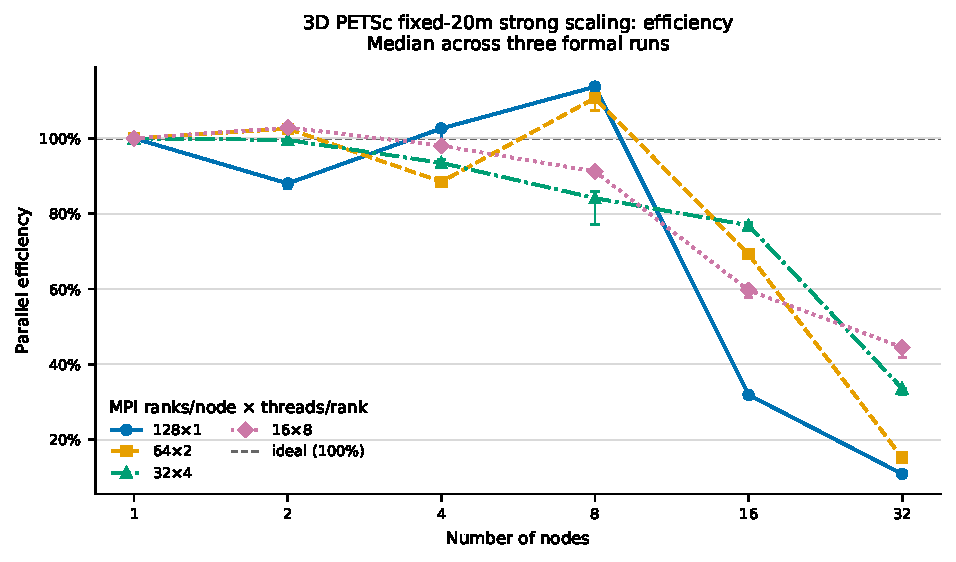
\includegraphics[width=0.85\textwidth]{figures/ksp3d_strong20m_efficiency}
  \caption{3D parallel efficiency at a fixed 20.35M unknowns, each layout against its own
  one-node time. This ranks scaling, not speed.}
  \label{fig:3d-strong20m-eff}
\end{figure}

\Cref{fig:3d-strong20m-eff} shows the same runs as parallel efficiency. Each layout is
measured against its own one-node time, so it ranks scaling and not speed. No 2D
counterpart is drawn, because the 2D curves do not turn over.

\subsection{Endpoints}
\label{sec:strong-endpoints}
\Cref{tab:strong20m-best} gives the fastest layout at each node count. In 2D the margin
over flat MPI never exceeds 6.9\%. In 3D it reaches 172.4\% at 16 nodes and 281.3\% at 32.

\begin{table}[htbp]
  \centering
  \caption{Fastest full-node layout at each node count for the fixed 20M problems, with its
  advantage over flat MPI.}
  \label{tab:strong20m-best}
  \begin{tabular}{lrlrrlrr}
    \toprule
    & & \multicolumn{3}{c}{2D, $4500^2$} & \multicolumn{3}{c}{3D, $273^3$} \\
    \cmidrule(lr){3-5}\cmidrule(lr){6-8}
    Nodes & Cores & Best & s/solve & vs.\ MPI & Best & s/solve & vs.\ MPI \\
    \midrule
     1 &  128 & $128\times1$ & 0.7704 &  0.0\% & $32\times4$ & 0.8022 &  13.0\% \\
     2 &  256 & $64\times2$  & 0.3365 &  1.0\% & $32\times4$ & 0.4028 &  27.8\% \\
     4 &  512 & $64\times2$  & 0.1265 &  6.9\% & $32\times4$ & 0.2145 &   2.9\% \\
     8 & 1024 & $64\times2$  & 0.0541 &  3.3\% & $64\times2$ & 0.0936 &   6.5\% \\
    16 & 2048 & $128\times1$ & 0.0313 &  0.0\% & $32\times4$ & 0.0652 & 172.4\% \\
    32 & 4096 & $64\times2$  & 0.0277 &  1.9\% & $16\times8$ & 0.0681 & 281.3\% \\
    \bottomrule
  \end{tabular}
\end{table}

\Cref{tab:strong20m-endpoints} gives all four layouts at 32 nodes. The 2D speedups are
almost equal, 27.3 to 29.8, because each layout is measured against its own one-node time
and $16\times8$ starts from the worst one. Their runtimes still differ by 45\%. In 3D the
two measures agree, because the layouts diverge instead of converging.

\begin{table}[htbp]
  \centering
  \caption{The 32-node endpoint of the fixed-size curves. Only time per solve compares layouts
  directly.}
  \label{tab:strong20m-endpoints}
  \begin{tabular}{llrrrr}
    \toprule
    Case & Layout & s/solve & Speedup & Efficiency & 16$\to$32 step \\
    \midrule
    2D & $128\times1$ & 0.0282 & 27.30 & 85.3\% & 55.5\% \\
    2D & $64\times2$  & 0.0277 & 29.83 & 93.2\% & 62.9\% \\
    2D & $32\times4$  & 0.0317 & 27.85 & 87.0\% & 61.1\% \\
    2D & $16\times8$  & 0.0409 & 27.71 & 86.6\% & 69.4\% \\
    \addlinespace
    3D & $128\times1$ & 0.2599 &  3.49 & 10.9\% & 34.2\% \\
    3D & $64\times2$  & 0.1703 &  4.87 & 15.2\% & 22.0\% \\
    3D & $32\times4$  & 0.0747 & 10.75 & 33.6\% & 43.7\% \\
    3D & $16\times8$  & 0.0681 & 14.24 & 44.5\% & 74.6\% \\
    \bottomrule
  \end{tabular}
\end{table}

\section{Interpretation}
\label{sec:mn-interp}
\Cref{tab:cross-dimension} collects the comparison. It gives both a throughput gain and
a time saving, because these are different conventions and the chapter quotes both. The
two halves do not carry equal weight. The 3D gaps over flat MPI at 16 and 32 nodes, $2.72\times$ and $3.81\times$, are
far outside the run-to-run spread. The 1--7\% margins the 2D layouts hold on the fixed
problem are not, so the 2D ordering at any single node count is only indicative.

\begin{table}[htbp]
  \centering
  \caption{The two dimensions on the quantities this chapter compares them by.}
  \label{tab:cross-dimension}
  \begin{tabular}{lll}
    \toprule
    & 2D & 3D \\
    \midrule
    \multicolumn{3}{l}{\emph{Constant work per core, 11 size--node pairs}} \\
    Layout winning most points        & $64\times2$ (8 of 11) & $32\times4$ (6 of 11) \\
    Hybrid points faster per iteration & 13 of 33 & 22 of 33 \\
    Largest throughput gain           & 14.7\% & 33.2\% \\
    Largest per-iteration saving      & 12.8\% & 24.9\% \\
    Ratio series monotone in nodes    & 4 of 6 & 0 of 6 \\
    Weak efficiency rises with threads & yes & no \\
    \addlinespace
    \multicolumn{3}{l}{\emph{Fixed 20M problem, one to 32 nodes}} \\
    Layouts that saturate by 32 nodes & none of 4 & 3 of 4 \\
    First to saturate                 & --- & $128\times1$, at 8 nodes \\
    Fastest at 32 nodes               & $64\times2$ & $16\times8$ \\
    Its lead over flat MPI            & $1.02\times$ & $3.81\times$ \\
    Fastest-to-slowest spread there   & $1.48\times$ & $3.81\times$ \\
    \bottomrule
  \end{tabular}
\end{table}

2D is ordered and 3D is not. Every 2D hybrid layout improves against flat MPI as
concurrency grows, and weak efficiency rises with threads per rank. In 3D the margins are
about twice as large, but no series is monotone and the best layout changes with scale and
node count.

The regime matters as much as the dimension. At constant work per core the layout effect
is a few per cent. At constant problem size it is unbounded, because the layouts differ in
where they stop scaling rather than in speed.

The two stencils do different work per equation, so their absolute rates are not a
comparison of algorithms. What compares is the layout ordering and the margin over flat
MPI.

Two results here are not explained here. The first is the 2D ordering. Adding threads
helps more as concurrency grows, which is what a communication-share account would
predict. This chapter measures runtime and not communication, so it cannot test that
account. The second is $16\times8$. It removes the most MPI endpoints of any layout and is
still the slowest 2D layout at all 11 points. Whatever hybridisation saves, it also costs
something that grows with the thread count. \Cref{ch:profiling} measures both directly.

What this chapter does settle is that a layout recommendation needs the regime it was
measured in. $16\times8$ is last at constant work per core in both dimensions and first at
4096 cores on the fixed 3D problem, by $3.81\times$. Both readings are right. They answer
different questions.


\chapter{Profiling and Bottleneck Analysis}
\label{ch:profiling}
\section{Why a Repeated-Solve Driver}
\label{sec:whyrepeat}
In a single solve at 20.25M with $16\times8$, \texttt{-log\_view} gave \texttt{PCSetUp}
45\% of time and \texttt{KSPSolve} 10\%. \texttt{ex2\_repeat} runs the solve inside a
\texttt{RepeatedSolves} log stage, zeroes the initial guess before each solve, and reuses
the preconditioner (\texttt{-ksp\_reuse\_preconditioner} and
\texttt{-pc\_gamg\_reuse\_interpolation true}). With 20 solves the stage held 69\% of time
and 93\% of flops; within the stage \texttt{KSPSolve} was 100\% of time; each of the 19
repeats took 11 iterations. The corrected scaling campaign uses this same warm-up and
reuse design, so \Cref{ch:multinode} compares steady-state solves rather than first-touch
and hierarchy-construction costs.

\section{Analysis Methodology}
\label{sec:analysis-method}
The method combines MAP 25.0.4 timelines with \texttt{-log\_view} \%T (share of stage
time) and \%F (share of stage flops). An event whose \%T exceeds its \%F spends the
difference on communication, synchronisation, or memory traffic. \Cref{tab:tf} lists
single-point data for the RepeatedSolves stage at 20.25M with $16\times8$.

\begin{table}[htbp]
  \centering
  \caption{Per-event time and flop shares, RepeatedSolves stage, 20.25M, $16\times8$.}
  \label{tab:tf}
  \begin{tabular}{lrrr}
    \toprule
    Event & \%T & \%F & GF/s \\
    \midrule
    \texttt{MatMult}          & 39 & 55 & 30.5 \\
    \texttt{MatMultTranspose} & 18 &  6 &  6.7 \\
    \texttt{VecTDot+VecNorm}  &  8 &  6 & --   \\
    \texttt{PCApply} (agg.)   & 82 & 82 & 21.6 \\
    \bottomrule
  \end{tabular}
\end{table}

\texttt{MatMultTranspose} (GAMG restriction) has a \%T three times its \%F and a rate
$4.6\times$ below \texttt{MatMult}. \texttt{VecTDot} and \texttt{VecNorm} are the CG global
reductions.

\section{MAP Profiling Results}






\begin{table}[htbp]
  \centering
  \caption{Share of total core-time inside the solve window, by the library owning the
  executing frame, for the eleven usable MAP profiles at 20.25M unknowns in 2D.}
  \label{tab:map-shares}
  \begin{tabular}{llrrrrr}
    \toprule
    Build & Nodes & Layout & PETSc & OpenMP & MPI & LibSci \\
    \midrule
    LibSci   &  2 & $64\times2$ & 31.9\% & 36.5\% & 29.9\% & 1.0\% \\
    LibSci   &  2 & $32\times4$ & 51.6\% & 40.1\% &  5.8\% & 1.7\% \\
    LibSci   &  2 & $16\times8$ & 42.2\% & 53.5\% &  1.4\% & 2.1\% \\
    \addlinespace
    LibSci   &  8 & $64\times2$ &  4.5\% & 48.3\% & 46.7\% & 0.2\% \\
    LibSci   &  8 & $32\times4$ &  7.5\% & 69.3\% & 22.6\% & 0.3\% \\
    LibSci   &  8 & $16\times8$ & 15.6\% & 76.5\% &  6.2\% & 1.0\% \\
    \addlinespace
    Baseline &  2 & $32\times4$ & 51.7\% & 40.8\% &  6.7\% & 0.0\% \\
    Baseline &  2 & $16\times8$ & 40.2\% & 57.8\% &  1.4\% & 0.0\% \\
    Baseline &  8 & $32\times4$ &  8.8\% & 68.6\% & 22.2\% & 0.0\% \\
    Baseline &  8 & $16\times8$ & 16.0\% & 77.5\% &  6.0\% & 0.0\% \\
    Baseline & 16 & $32\times4$ &  1.2\% & 69.8\% & 29.0\% & 0.0\% \\
    \bottomrule
  \end{tabular}
\end{table}


\begin{figure}[htbp]
  \centering
  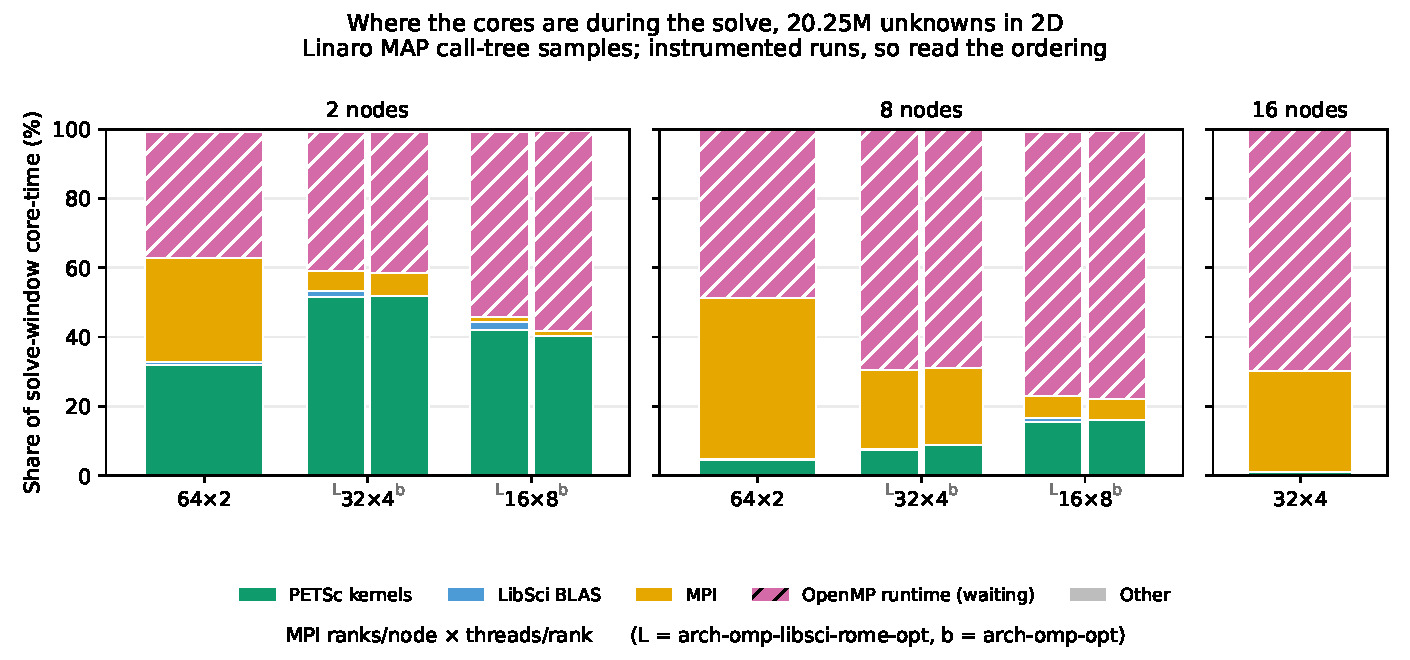
\includegraphics[width=\textwidth]{figures/map_solve_window_shares}
  \caption{Where the cores are during the solve, from the MAP call trees. }
  \label{fig:map-shares}
\end{figure}


\section{Bottleneck Identification}

\begin{figure}[htbp]
  \centering
  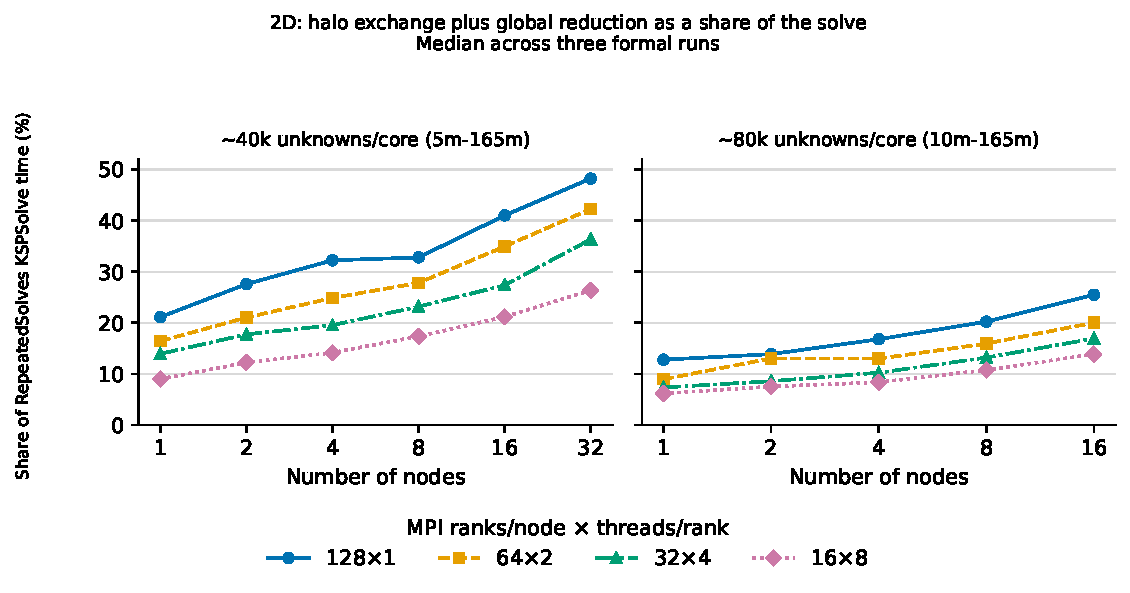
\includegraphics[width=0.85\textwidth]{figures/ksp2d_sync_share}
  \caption{2D share of \texttt{RepeatedSolves} \texttt{KSPSolve} time spent inside halo
  exchange and global reduction events. The ordering matches the time-per-iteration
  ordering in \Cref{fig:2d-ratio} at every node count.}
  \label{fig:2d-sync}
\end{figure}

\begin{figure}[htbp]
  \centering
  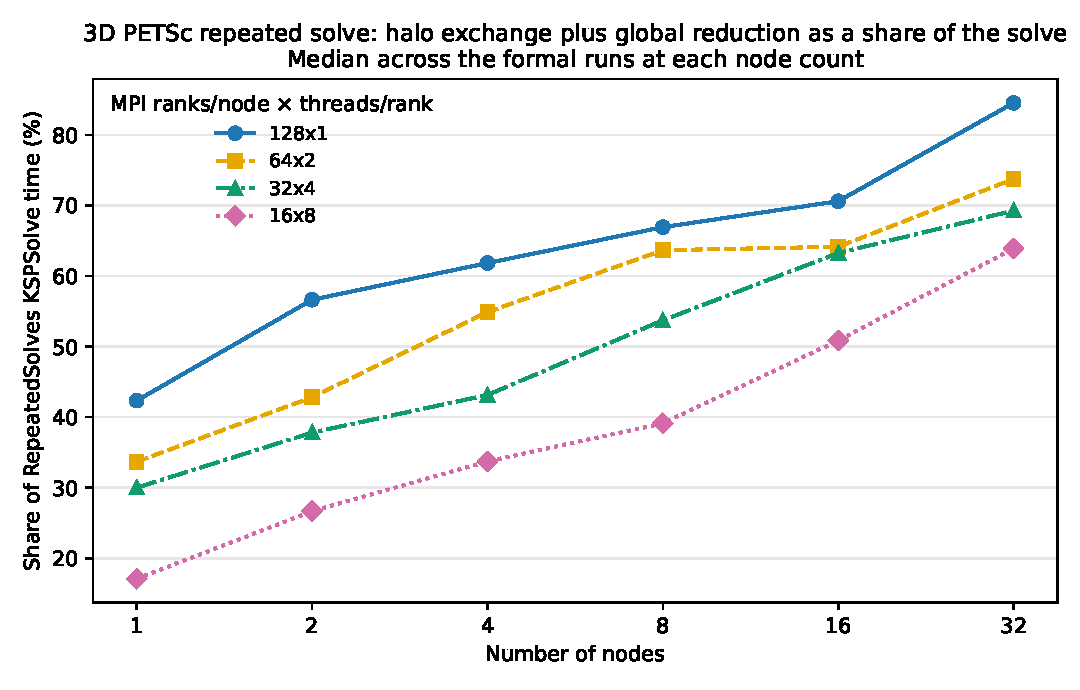
\includegraphics[width=0.85\textwidth]{figures/ksp3d_sync_share}
  \caption{3D share of \texttt{RepeatedSolves} \texttt{KSPSolve} time spent inside halo
  exchange and global reduction events. Note the vertical scale: flat MPI reaches 84.6\%
  at the largest point.}
  \label{fig:3d-sync}
\end{figure}


\chapter{Discussion}


\chapter{Conclusion and Future Work}
%%%%%%%%%%%%%%%%%%%%%%%%%%%%%%%%%%%%%%%%%%%%%%%%%%%%%%%%%%%%%%%%%%%%%%%%%%%%%%%
%%% Appendix
%%%%%%%%%%%%%%%%%%%%%%%%%%%%%%%%%%%%%%%%%%%%%%%%%%%%%%%%%%%%%%%%%%%%%%%%%%%%%%%
\appendix
% The appendix command just changes heading styles for appendices.

\chapter{Supplementary Figures}
\label{app:figures}
\Cref{fig:2d-throughput} and \Cref{fig:3d-throughput} give raw repeated-solve throughput
for the weak-scaling campaign of \Cref{sec:weak}. Throughput rises almost linearly with
the node count along both chains in both dimensions. The four layouts differ by only a few
per cent against a range of three orders of magnitude, so these figures cannot carry the
layout comparison. \Cref{fig:2d-ratio} and \Cref{fig:3d-ratio} do that instead.

\begin{figure}[htbp]
  \centering
  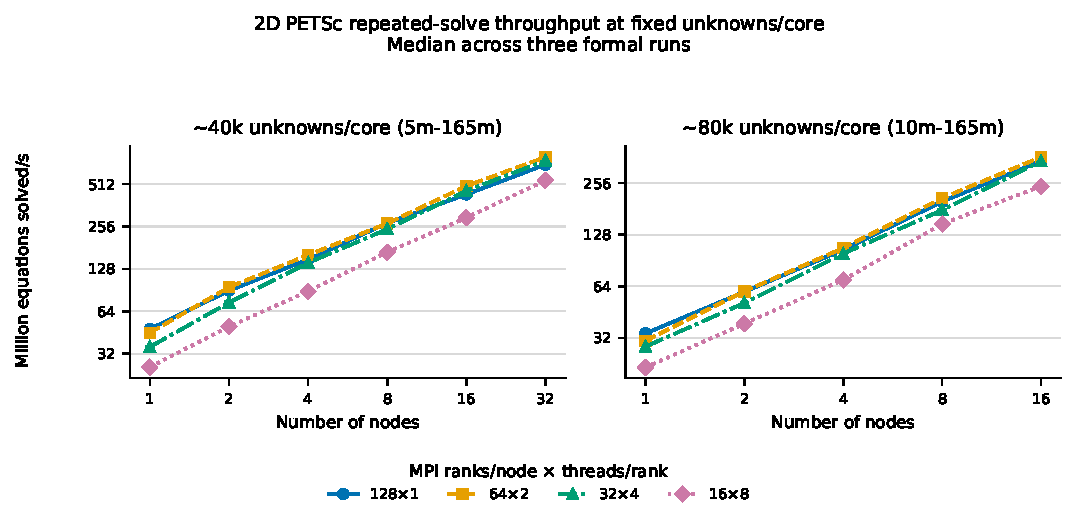
\includegraphics[width=\textwidth]{figures/ksp2d_throughput_vs_nodes}
  \caption{Median 2D repeated-solve throughput along the two unknowns/core chains.}
  \label{fig:2d-throughput}
\end{figure}

\begin{figure}[htbp]
  \centering
  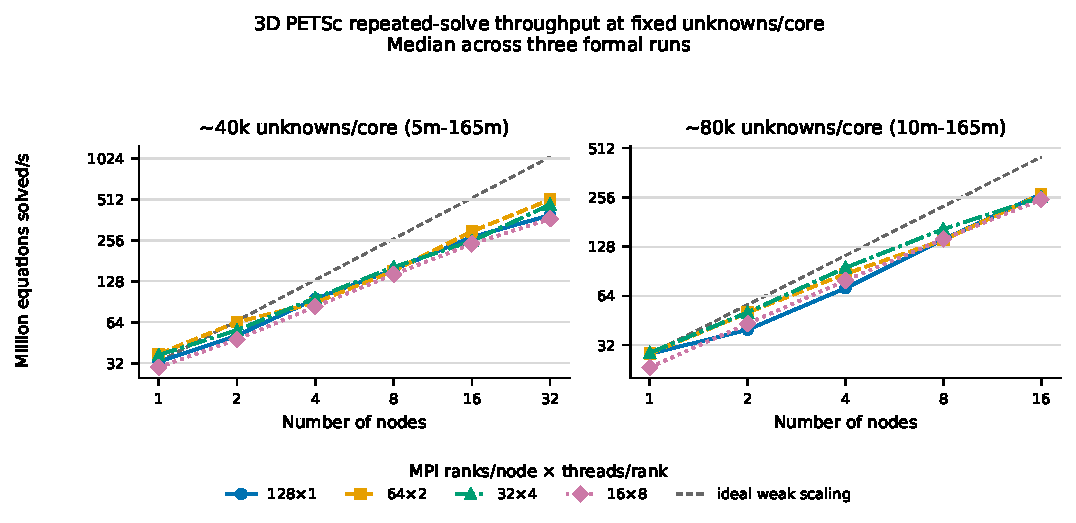
\includegraphics[width=\textwidth]{figures/ksp3d_throughput_vs_nodes}
  \caption{Median 3D repeated-solve throughput along the two unknowns/core chains.}
  \label{fig:3d-throughput}
\end{figure}

\chapter{Stuff which is too detailed}

Appendices should contain all the material which is considered too
detailed to be included in the main body but which is, nevertheless,
important enough to be included in the thesis.

\chapter{Stuff which no-one will read}

Some people include in their thesis a lot of detail, particularly
computer code, which no-one will ever read. You should be careful that
anything like this you include should contain some element of uniqueness
which justifies its inclusion.

%%%%%%%%%%%%%%%%%%%%%%%%%%%%%%%%%%%%%%%%%%%%%%%%%%%%%%%%%%%%%%%%%%%%%%%%%%%%%%%
%%% Bibliography
%%%%%%%%%%%%%%%%%%%%%%%%%%%%%%%%%%%%%%%%%%%%%%%%%%%%%%%%%%%%%%%%%%%%%%%%%%%%%%%

\printbibliography


\end{document}




\title{Hybrid MPI+OpenMP Performance of PETSc Krylov Solvers on ARCHER2}
\author{Leyan Li}
\date{August 2026}

\makeEPCCtitle
% This takes care of creating all the logos on the title page as described in
% epcc.sty --- feel free to explore it!

\thispagestyle{empty} 
% We don't want any page numbers, headers or footers on the title page,
% hence "empty" style.

% The below is a dirty way of adding all the relevant degree- and university- 
% information onto the title page. Sorry.
%
\vspace{9cm} % This controls the amount of vertical space between the title and 
			 % your name, and the degree information. The University, degree and 
			 % year should show at the bottom of the page so please adjust 
			 % the vspace accordingly, to avoid it overflowing onto the next page.

\begin{center}

% Adjust the information below to fit your situation. If anything takes more 
% space than expected in the template, adjust spacing above/below to keep all
% this on the first page.
\large{MSc in High Performance Computing (with Data Science)} \\ 
	% update based on your degree
\large{The University of Edinburgh} \\ %
\large{Year} \\ % update to the year you are submitting your dissertation 

\end{center}

% This is it, the title page is done. Go you!

% We are starting to number pages from here, right after the title page.
% These are non-technical content pages, and these are 
% number them with roman numerals. Content pages (starting from
% Chapter 1) will get numbered with arabic numerals, restarting from '1'.
\pagenumbering{roman}
\setcounter{page}{0}
\newpage

% We used the "abstract" style common in research publications and
% therefore use the predefined LaTeX macro. However, we want this page
% to be numbered with 'i' (first page after the title), so we need to
% overwrite the page style to show page numbers, adding 
% \thispagestyle{plain} **inside** the abstract.
\begin{abstract} 
\thispagestyle{plain}
\noindent This is the bit where you summarise what is in your thesis. A non-expert reader 
should be able to understand the area of your work, what the main challenges 
were and what contributions or insights you've achieved, and gauge whether 
this work is relevant to their interests,. Think of the abstract as 
a super-concentrated summary of your MSc project; advertise your work 
but try to avoid cliffhangers.

A good abstract fits to 1 to 2 paragraphs and takes around 200 words to get your 
point across. To give you an idea, this abstract is 97 words long.
\end{abstract}

% The following commands generate pages of non-technical content; as the names 
% suggest, we will generate tables of content, of tables and of figures. It is 
% recommended that you have a look at these tables and decide whether they are 
% displayed correctly with a meaningful amount of information (for example,
% list of figures should not contain the full figure captions), and whether 
% they are relevant and needed.
%
\tableofcontents
\listoftables
\listoffigures

% You may decide to include additional sections, for example the 
% Acknowledgements or Dedications. Make sure these start on a new page, 
% following the structure below:
\newpage

% This vspace is just to avoid having a short amount of text 
% (the Acknowledgements) hanging awkwardly at the very top of the page.
\vspace*{2in}

\section*{Acknowledgements}

Here you can give credit to anyone who has enabled the progress of your MSc 
project, especially if this was \emph{above and beyond} their role. Below is 
our acknowledgement of the people who contributed to creation of this template. 
\\ \\
%
This template is a slightly modified version of the one developed by
Prof. Charles Duncan for MSc students in the Dept. of Meteorology. His
acknowledgement follows:

\emph{This template has been produced with help from many former students who
have shown different ways of doing things. Please make suggestions for
further improvements.} 

% This is the end of the "initial matters", the technical content follows
% from here. The page numbering is restarted and arabic style invoked 
% by the command below.
%




%%%%%%%%%%%%%%%%%%%%%%%%%%%%%%%%%%%%%%%%%%%%%%%%%%%%%%%%%%%%%%%%%%%%%%%%%%%%%%%
%%% Appendix
%%%%%%%%%%%%%%%%%%%%%%%%%%%%%%%%%%%%%%%%%%%%%%%%%%%%%%%%%%%%%%%%%%%%%%%%%%%%%%%
\appendix
% The appendix command just changes heading styles for appendices.

\chapter{Stuff which is too detailed}

Appendices should contain all the material which is considered too
detailed to be included in the main body but which is, nevertheless,
important enough to be included in the thesis.

\chapter{Stuff which no-one will read}

Some people include in their thesis a lot of detail, particularly
computer code, which no-one will ever read. You should be careful that
anything like this you include should contain some element of uniqueness
which justifies its inclusion.

%%%%%%%%%%%%%%%%%%%%%%%%%%%%%%%%%%%%%%%%%%%%%%%%%%%%%%%%%%%%%%%%%%%%%%%%%%%%%%%
%%% Bibliography
%%%%%%%%%%%%%%%%%%%%%%%%%%%%%%%%%%%%%%%%%%%%%%%%%%%%%%%%%%%%%%%%%%%%%%%%%%%%%%%

\begin{thebibliography}{100}

\bibitem{ref:lam} L.~Lamport. {\em Latex User's Guide
and Reference Manual.\\} Addison Wesley, 1986, pp242.

\bibitem{ref:bloggs} F.~Bloggs. {\em Latex Users do it
in Environments.\\} Int. Journal of Silly Findings, 1993, pp 23-29.

\end{thebibliography}


\end{document}
